\documentclass[12pt,twoside]{article}
%\date{}   %uncommenting this erases the date
\usepackage{graphicx}
\usepackage{amsmath}
\usepackage{amssymb}
%\usepackage{natbib}
%\usepackage{verbatim}
\usepackage{floatpag}
\usepackage{subeqnarray}
\usepackage{mathrsfs}    %for special characters
\usepackage{cancel}  % to set terms in an equation to zero



\setlength{\textheight}     {9.0in}
\setlength{\textwidth}      {6.5in}
\setlength{\oddsidemargin}  {0.0in}
\setlength{\evensidemargin} {0.0in}
\setlength{\topmargin}      {0.0in}
\setlength{\headheight}     {0.0in}
\setlength{\headsep}        {0.0in}
\setlength{\hoffset}        {0.0in}
\setlength{\voffset}        {0.0in}
\setlength{\parindent}      {0.0in}      %starting new line at extreme left

\graphicspath{{Figures/}}

\newcommand{\astrut}{\usebox{\astrutbox}}

\newcommand\GaPQ{\ensuremath{G_a(P,Q)}}
\newcommand\GsPQ{\ensuremath{G_s(P,Q)}}
\newcommand\p{\ensuremath{\partial}}
\newcommand\tti{\ensuremath{\rightarrow\infty}}
\newcommand\kgd{\ensuremath{k\gamma d}}
\newcommand\shalf{\ensuremath{{\scriptstyle\frac{1}{2}}}}
\newcommand\sh{\ensuremath{^{\shalf}}}
\newcommand\smh{\ensuremath{^{-\shalf}}}
\newcommand\squart{\ensuremath{{\textstyle\frac{1}{4}}}}
\newcommand\thalf{\ensuremath{{\textstyle\frac{1}{2}}}}
\newcommand\Gat{\ensuremath{\widetilde{G_a}}}
\newcommand\ttz{\ensuremath{\rightarrow 0}}
\newcommand\ndq{\ensuremath{\frac{\mbox{$\partial$}}{\mbox{$\partial$} n_q}}}
\newcommand\sumjm{\ensuremath{\sum_{j=1}^{M}}}
\newcommand\pvi{\ensuremath{\int_0^{\infty}%
  \mskip \ifCUPmtlplainloaded -30mu\else -33mu\fi -\quad}}

\newcommand\etal{\mbox{\textit{et al.}}}
\newcommand\etc{etc.\ }
\newcommand\eg{e.g.\ }



\newcommand{\bs}  [1]{\boldsymbol{#1}}
\newcommand{\del} {\nabla}
\newcommand{\bsh}  [1]{\boldsymbol{\hat{#1}}}
\newcommand{\ul}  {\underline}
\newcommand{\ol}  {\overline}
\newcommand{\pp} [2]{\frac{\p{#1}}{\p{#2}}}
\newcommand{\dd} [2]{\frac{d{#1}}{d{#2}}}
\newcommand{\lam}  [1]{{#1}^{\tiny{\lambda}}}
\newcommand{\conj} [1]{{#1}^*}
\newcommand{\mods} [1]{ \vert {#1} \vert ^2}


\begin{document}

\title{Truncated 1-D Shallow Water Equations}


\author{Raghav Singhal}

\maketitle
In this work we trace the interaction of 3 wavenumbers  $\alpha=1 ,\  \beta=1 ,\ \gamma=2$ which correspond to 2 waves and a vortex respectively. The initial conditions,$ \ t=0$ are :

\begin{align}
&h_\alpha=2 , \ h_\beta=3, \ h_\gamma=5
\\
&u_\alpha=\frac{\omega}{\alpha}h_\alpha , \ u_\beta=\frac{-\omega}{\beta}h_\beta, \ u_\gamma=0
\\
&v_\alpha=\frac{1}{i \alpha}h_\alpha , \ v_\beta=\frac{1}{i \beta}h_\beta , \ v_\gamma=i \gamma h_\gamma
\\
&\omega=\sqrt{1+\alpha^2}=2
\end{align}

Below we plot the potential vorticity with no waves in the initial conditions and another set with waves in the initial conditions, the potential vorticity is computed as follows:
\begin{align}
&q_\alpha=i \alpha v_\alpha - h_\alpha
\\
&q_\beta=i \beta v_\beta - h_\beta
\\
&q_\gamma=i \gamma v_\gamma - h_\gamma
\end{align}

\begin{figure}[ht]
\centering
\begin{minipage}[b]{0.45\linewidth}
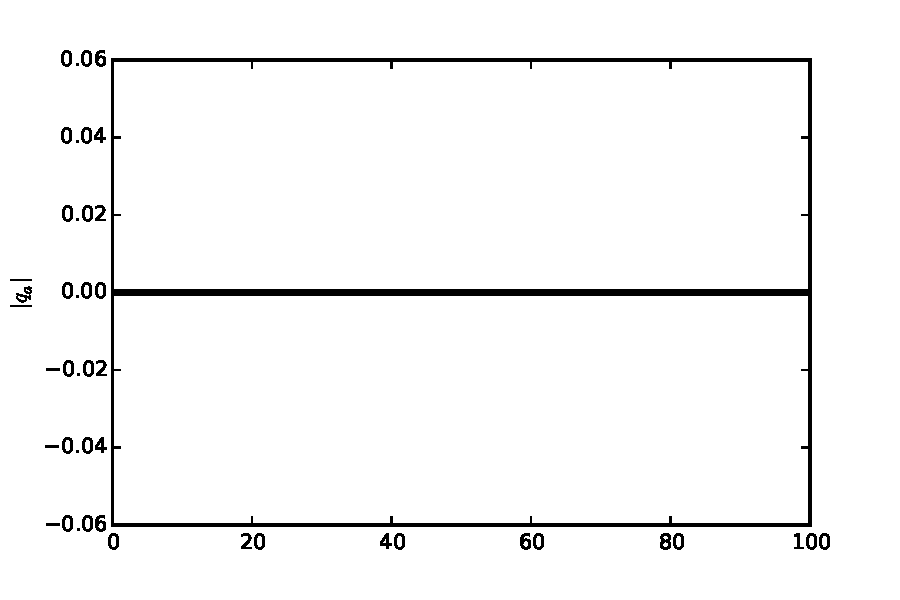
\includegraphics[width=3.2in,height=2.5in]{qa_nowave.pdf}
\caption{$q_\alpha$}
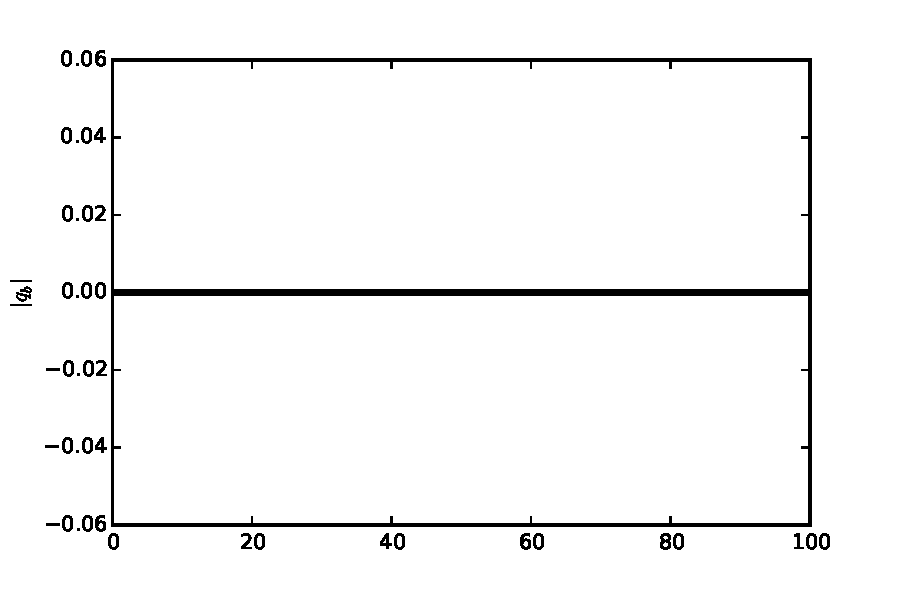
\includegraphics[width=3.2in,height=2.5in]{qb_nowave.pdf}
\caption{$q_\beta$}
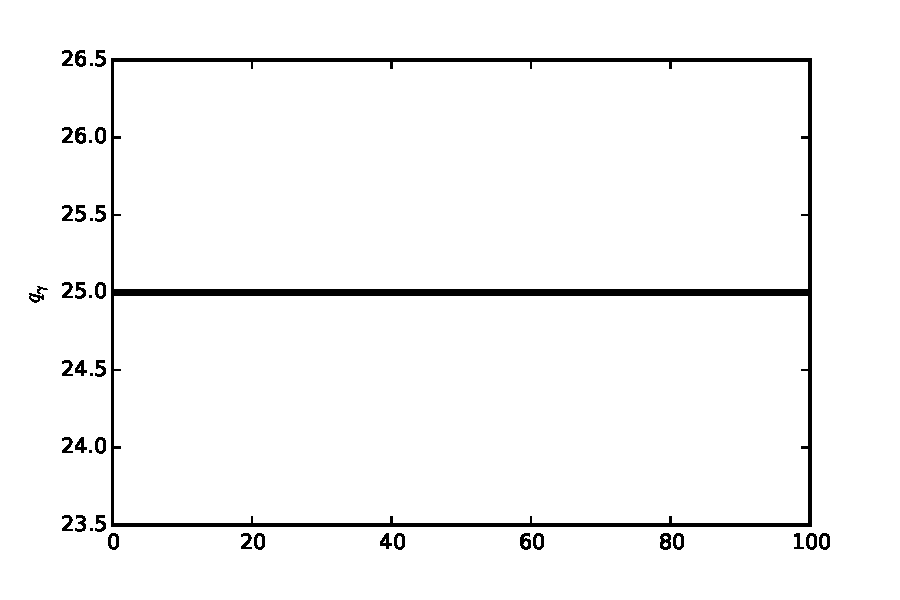
\includegraphics[width=3.2in,height=2.5in]{qg_nowave.pdf}
\caption{$q_\gamma$}

\caption{$\epsilon=0.05 ,\  t=100$, $with\ no \ waves \ in\ the\ initial\ conditions$}\end{minipage}
\quad
\begin{minipage}[b]{0.45\linewidth}

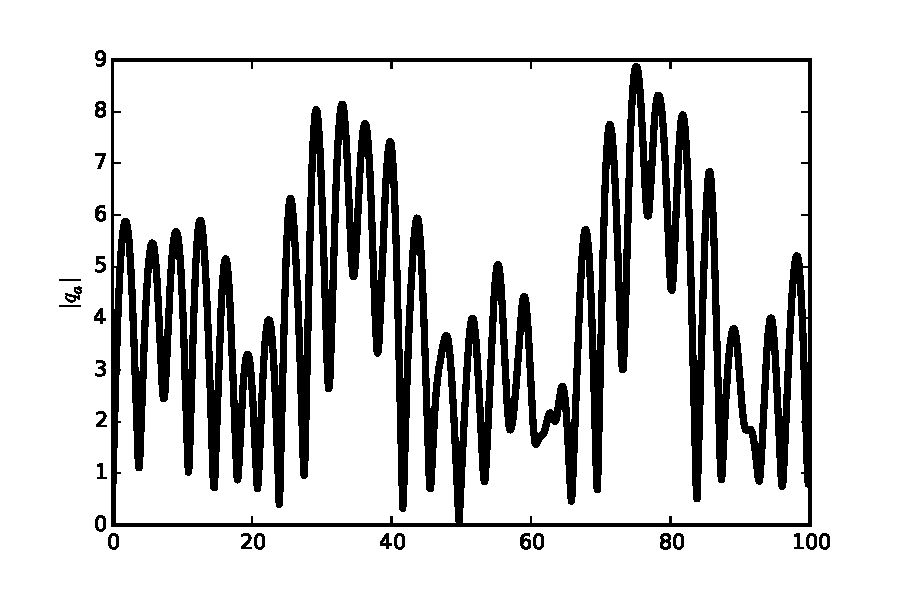
\includegraphics[width=3.2in,height=2.5in]{qa_wave.pdf}
\caption{$q_\alpha$}

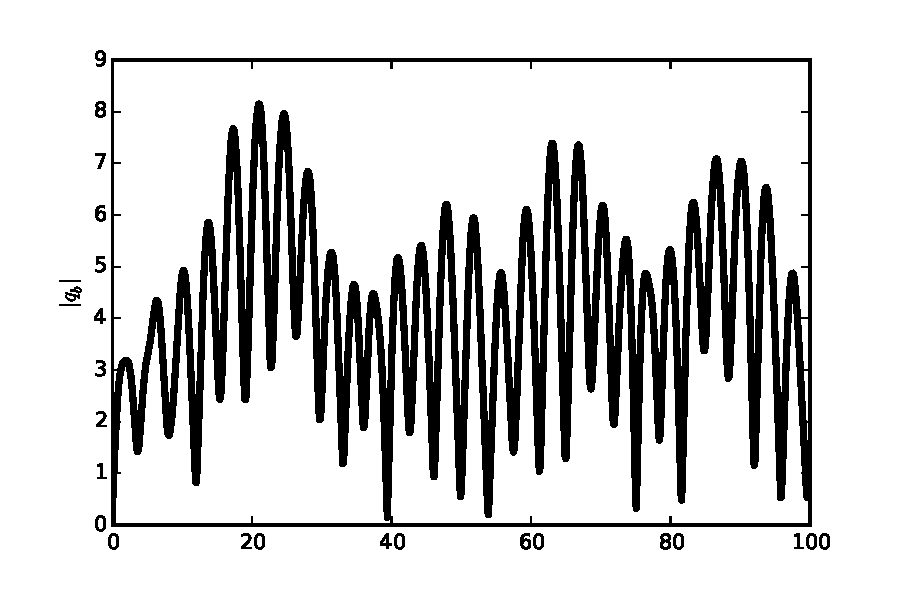
\includegraphics[width=3.2in,height=2.5in]{qb_wave.pdf}
\caption{$q_\beta$}

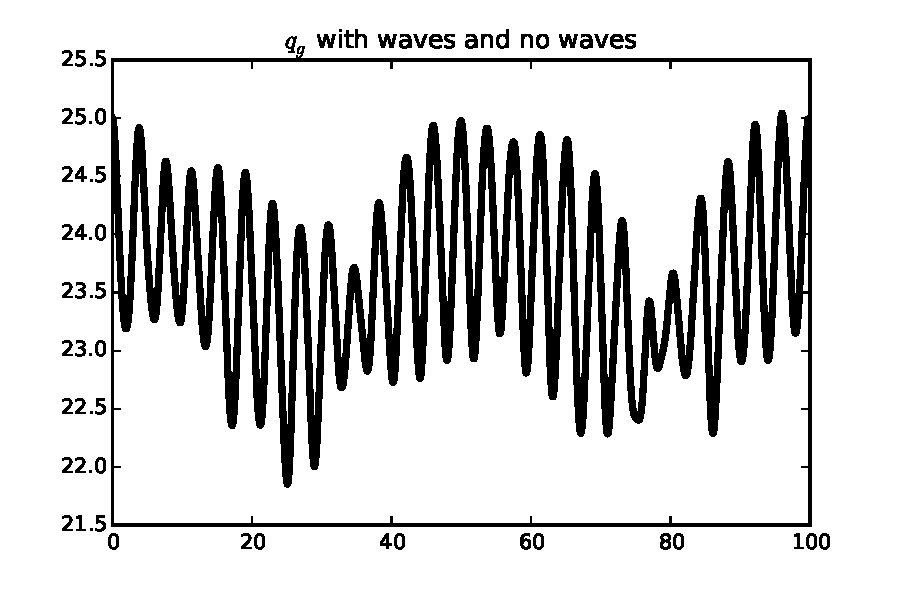
\includegraphics[width=3.2in,height=2.5in]{qg_wave.pdf}
\caption{$q_\gamma$}

\caption{$\epsilon=0.05 ,\  t=100$, $with\ waves \ in\ the\ initial\ conditions$}


\end{minipage}
\end{figure}
\clearpage
Below we plot the time-average of the potential vorticity of $q_\gamma$ and the evolution of $q_\gamma$ over time, in case of waves in the initial conditions and no waves in the initial conditions. The time average is calculated as follows:
\begin{equation}
Q_\gamma(t)=\frac{0.01 \epsilon}{2 \pi} \int_{t}^{t + \frac{2 \pi}{0.01 \epsilon}}q_\gamma(t) dt
\end{equation}
\begin{figure}

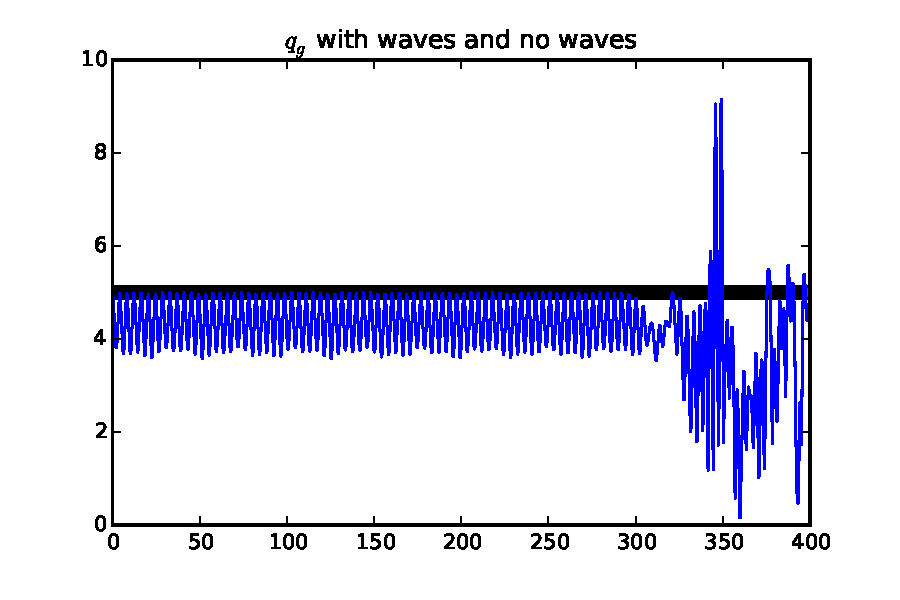
\includegraphics[width=8in,height=3.5in]{qg_e01.pdf}

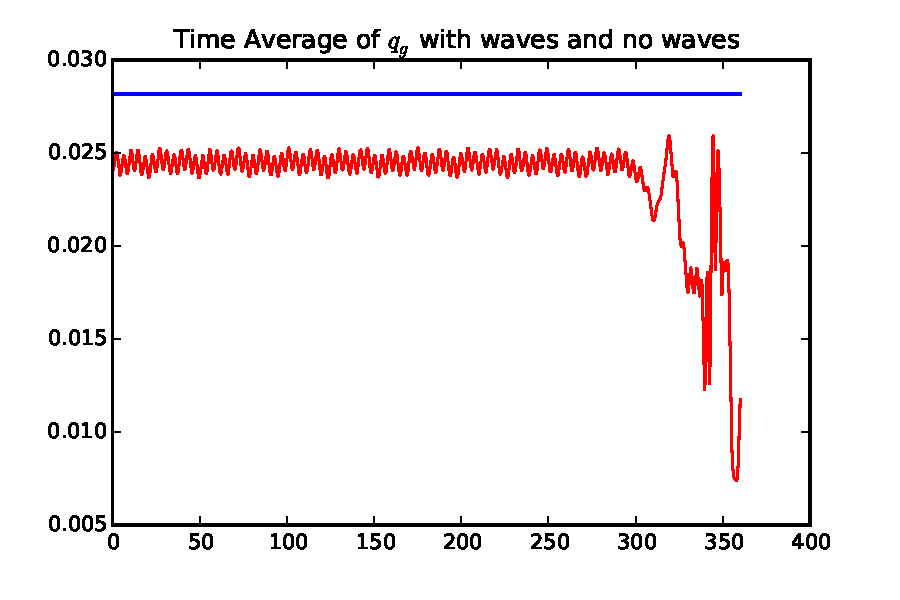
\includegraphics[width=8in,height=3.5in]{TimeAverage_e01.pdf}
\caption{$\epsilon=0.1 ,\  t=1000$}

\end{figure}

\end{document}